\pagestyle{plain} 

%\addcontentsline{toc}{chapter}{Lista de Figuras}
%\listoffigures
%\addcontentsline{toc}{chapter}{Lista de Tabelas}
%\listoftables

%################################################################################
\newcommand{\R}[1]{\ensuremath{\mathbb{R}^{#1}}}
\newcommand{\DB}{\ensuremath{\mathcal{D}}}
%comandos para as variaveis

\chapter{Introdução}
\label{cap-introducao}

Visualização é uma área da comunicação de informações que utiliza representações gráficas para extrair informações de conjuntos de dados\cite{ward2010interactive}, ela facilita a interpretação das informações, pois, fornece ao usuário modelos gráficos dos dados que podem ser interpretados mais rápidamente do fazendo uma analise dos dados brutos. Ela pode contribuir com diversas áreas de estudo como, finanças, esporte, politica, acadêmica, entre outras.

O foco deste projeto é a área acadêmica, pois, explorar coleções de documentos com o objetivo de identificar e extrair informações de interesse, como, uma revisão bibliográfica sistemática para uma pesquisa, exige muito tempo devido a necessidade de fazer uma seleção entre inúmeros artigos para descobrir quais são os mais relevantes à um determinado assunto. Em função ao aumento da produção textual nos últimos anos, como por exemplo no banco de dados de artigos da IEEE, fazendo-se uma busca rápida pelo termo \emph{"visualisation"}, até 2010 haviam aproximadamente 89 mil artigos científicos publicados, já no inicio de 2016 são mais de 159 mil \cite{IEEEsearch}, com base nesta informação há um aumento percentual de aproximadamente 79\%, com isso ter uma ferramenta que possa trabalhar com uma quantidade grande de artigos se torna necessária.

A efetividade da ferramenta utilizada depende muito da metáfora de visualização empregada para sintetizar e transmitir informações que se deseja conseguir a partir da visualização é muito importante para a interpretação por parte do usuário \cite{pagliosa2013mist}. Dentre diversas técnicas algumas são melhores para determinadas situações do que outras, como exemplo, nuvens de palavras é uma técnica eficaz em aplicações que se tem por finalidade fornecer uma visualização do resumo do conteúdo de documentos enquanto métodos que se baseiam em estruturas hierárquicas podem permitir uma exploração mais detalhada da relação entre documentos de acordo com a semelhança entre eles.

Varias metodologias propõem uma combinação de metáforas com o intuito de proporcionar um conjunto mais completo de informações em um único \emph{layout}.
 Embora algumas metáforas favoreçam a apresentação simultânea de informações com naturezas distintas, algumas abordagens existentes tem de fato sido bem sucedidas na criação de \emph{layouts} compostos que proporcionam efeitos visuais significativos, evitando representações que distraiam ou que sejam muito poluentes visualmente\cite{pagliosa2013mist}. Em particular, a combinação de layouts de pontos dinâmicos de dados textuais com base em conteúdo de sumarizações, tais como, nuvens de palavras é um problema que foi abordado por \cite{pagliosa2013mist}, mas, que precisa ser melhorado e estendido para se ter um aproveitamento efetivo da ferramenta.

 Este trabalho tem como finalidade fornecer uma ferramenta eficaz para realizar 

\section{Objetivos}
\label{Objetivos}

O objetivo geral deste projeto é o desenvolvimento de uma aplicação web para consulta visual de uma base de documentos que permita ao usuario realizar consultas e explorar o conteúdo resultante da visualização e a avaliação da tecnica por meio de testes de usuário.


O objetivo geral deste projeto é desenvolver uma estrutura teórica
computacional para exploração visual de uma base de dados composta por artigos científicos que permita o usuário realizar consultas e explorar o conteúdo resultante da visualização.

\subsection{Objetivos Especificos}
\label{ObjetivosEspecificos}

\begin{enumerate} %Começa uma lista
	\item Desenvolvimento do lado servidor da aplicação.
    \item Desenvolvimento do lado cliente
    \item Realizar testes com usuários 

\item Desenvolver uma ferramenta de visualização interativa baseada em projeções multidimensionais.
	\item Desenvolver uma aplicação capaz de trabalhar com uma base de dados extensível. 
	\item Desenvolver uma ferramenta que permita pesquisa, navegação na área de visualização.
	\item 
	\item 
		
	
\end{enumerate} % termina a lista
  
  
 


\section{Visão Geral para uso interno}
\label{usointerno}

O propósito deste trabalho é desenvolver um arcabouço teórico e
computacional para exploração visual da base de dados \DB.  A partir
de consultas feitas por um usuário (formulada em termos dos atributos dos
dados em \DB), a ferramenta resultante deve, primeiramente, selecionar
as $n_q$ instâncias oriundas do processamento da consulta para início
da exploração visual.  Em seguida, as $n_a\le n_q$ instâncias
selecionadas mais relevantes deverão ser mapeadas para um espaço
visual bidimensional, através do emprego de uma técnica de projeção
multidimensional.  Como decorrência da projeção, cada instância
selecionada $x_i$ será mapeada para um ponto $p_i\in\R{2}$. O próximo
passo é atribuir a cada ponto $p_i$ alguma forma geométrica de área
$a_i$ de acordo com ranqueamento de $x_i$, isto é, se
$r_{x_i}>r_{x_j}$, então $a_i>a_j$. O número $n_a$ é definido tal que
$$
\sum_{i=1}^{n_a} a_i < s_a\,A,
$$
%
em que $0<s_a\le 1$ é um fator especificado pelo usuário e $A$ é a
área da janela do espaço visual no qual a visualização será exibida.
Em virtude de formas geométricas serem atribuídas aos pontos
projetados, essas podem se interceptar no espaço visual.  Por isso,
deverá ser empregado algum método de repulsão que, ao mesmo tempo em
que evita a sobreposição das formas geométricas, mantém, tanto quanto
possível, a relação de vizinhança entre os pontos da projeção.  As
$n_q-n_a$ instâncias selecionadas restantes (isto é, que não têm área
associada) deverão ter seus pontos projetados exibidos utilizando-se
alguma metáfora representativa de alguma medida de \emph{densidade} no
espaço visual. Assim, áreas da janela de visualização com maior
``densidade'' de pontos representarão regiões com um número maior de
instâncias a serem exploradas pelo usuário. 


Usuário poderá interagir com os resultados da visualização, além de poder realizar consultas através de querys. Após o resultado visual da busca do usuário também poderá fazer seleção de áreas de interesse para explorar melhor a coleção de dados na tela.

As formas geométricas decorrentes da visualização deverão conter informações sobre os dados que elas representam com tags mostrando nome, autor e outras informações relevantes.

Sumario de um agrupamento


%Os objetivos específicos ainda estão sendo definidos.

Este trabalho será baseado em uma aplicação ja existente, desenvolvida por \cite{pagliosa2013mist} o MIST, este por sua vez tem funções limitadas que serão exploradas e poderão ser desenvolvidas com objetivos ampliados.

\section{MIST}
\label{mist}

O MIST \textit{(Multiscale Information and Summaries of Texts)} é uma ferramenta que permite a visualização simultânea de documentos individuais, bem como um resumo do conteúdo de coleções de documentos, permite uma exploração multi escalar de subconjuntos de documentos por conteúdo\cite{pagliosa2013mist}. 


\begin{figure}[!ht]
	\centering
	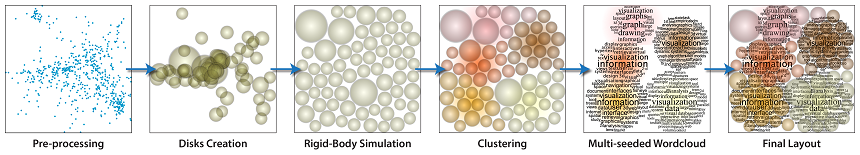
\includegraphics[width=1\columnwidth]{images/mist_pipeline.png}
	\caption{Pipeline de visualizações do MIST \cite{pagliosa2013mist}}
	\label{fig:MISTpipeline}
\end{figure}

A técnica MIST compreende três etapas principais: pré-processamento, criação de discos, simulação de corpo rígido e geração de nuvem de palavras, como ilustrado na Fig. \ref{fig:MISTpipeline}. Três tarefas são realizadas durante o pré-processamento. A primeira tarefa é um processo de extração de palavras-chave, para gerar a nuvem de palavras no terceiro passo do pipeline. Palavras-chave são também usadas para calcular a similaridade entre documentos. Esta semelhança é usada no segundo passo, como entrada para um processo de projeção multidimensional que mapeia os documentos em um espaço visual 2D. A importância de cada documento na coleção também é computada como uma pré-tarefa de processamento e é baseada na ligação entre os documentos individuais, dadas por um usuário ou aplicação definida. Na segunda etapa do MIST, uma simulação de motor de corpo rígido  organiza um conjunto de discos que representam os documentos, com o seu tamanho determinado pela importância do documento, evita também sobreposições e ainda preserva estruturas de vizinhança fornecidas pela projeção multidimensional inicial \cite{pagliosa2013mist}.
Na terceira e última etapa do pipeline, os documentos são agrupados de acordo com sua vizinhança, após isto, nuvens de palavras são geradas e harmoniosamente fundidas para produzir o layout final.

 Mas, a aplicação tem limitações como por exemplo a quantidade de artigos que podem ser processados (\textit{deadline:} 2 mil artigos), não sendo viável tratar uma quantia maior de artigos, entre outras que serão exploradas ao decorrer do trabalho. Para que a ferramenta seja usada para processar uma quantia maior de artigos terá de ser feita uma reestruturação de seus algoritmos e métodos.

Contexto e relevância (o que já existe atualmente: MIST).

Lacunas do MIST a serem investigadas no projeto:
\begin{itemize}
	\item Tamanho da base de dados \DB\ pode se tornar ``grande''. Como consequência, à medida que novas instâncias são adicionadas a \DB,
	tornam-se necessário o uso de um método de ranqueamento e de projeção
	multidimensional \emph{incrementais}. Atualmente, MIST emprega
	projeções que podem manipular somente conjuntos ``pequenos'' de
	dados.
	
	\item MIST não admite consultas iniciais.
	
	\item As formas geométricas em MIST são restritas a círculos.
	
	\item O método de repulsão é baseado em impulsos aplicados às formas
	geométricas, consideradas como sendo corpos rígidos
	bidimensionais. O método não consegue fazer uma escala eficiente para um número
	``grande'' de pontos.
	
	\item MIST não emprega uma metáfora para densidade de pontos.
	
	\item MIST não efetua agrupamentos no espaço \R{m}, mas sim no
	espaço visual \R{2}. O número de grupos é especificado
	arbitrariamente pelo usuário e computado através de
	\emph{k-means}. Como consequência, as instâncias em um agrupamento
	não mantêm necessariamente outra relação entre si que não seja a de
	proximidade de suas projeções no espaço visual.
	
	\item MIST sumariza um agrupamento através de nuvens de palavras, as quais são exibidas como textura de fundo do retângulo envolvente do agrupamento no espaço visual. Tal procedimento restringe o emprego	de sumários. Embora a visualização contenha vários elementos
	informativos, pode-se contestar a real eficácia de tal esquema de	sumarização, além da confusão visual por parte de usuários.
	
\end{itemize}



%##############################################################
\chapter{Trabalhos Relacionados e Fundamentos}
\label{cap-trab-relacionados}

\section{Introdução}
\label{intro_trab_relac}

Neste capítulo são apresentados os alguns trabalhos mais relevantes, métodos que são relacionados e conceitos teóricos necessários para o desenvolvimento deste trabalho como:
...

%-----------------------------------
\section{Trabalhos Relacionados}
\label{Trab_Relac}


Koh et. al. \cite{koh2010maniwordle} apresenta uma ferramenta de visualização de palavras baseada em Wordle (aplicação usada para gerar nuvens de palavras) o ManiWordle. Ele renova as interações com o layout, apoiando manipulações personalizadas, permite a manipulação de tipografia, cor e composição, não só para o layout como um todo, mas, também para as palavras individuais, permitindo ter um melhor controle sobre o resultado do layout. 

Wu et. al. \cite{wu2011semantic} apresenta um método para criar nuvens de palavras preservando a semântica, apresentando uma metodologia que calcula primeiro as relações semânticas e em seguida usa escalonamento multidimensional para colocar as palavras-chave no espaço visual.


Métodos, como SparkClouds apresentado em \cite{lee2010sparkclouds} e Tag Clouds Paralel \cite{collins2009parallel}, aumentam as nuvens de palavras com recursos visuais adicionais, tais como linhas de ignição e coordenadas paralelas, a fim de melhor transmitir o conteúdo do resumo de documentos. Embora muito eficaz para descobrir informações essenciais contidas em uma coleção de documentos, o paradigma da nuvem de palavras por si só não identifica a associação entre palavras para um determinado documento ou grupo de documentos e não permite o exame de similaridade entre eles.

Em \cite{joia2015uncovering} é proposta uma técnica de visualização multidimensional com projeção que se baseia em exemplos representativos para definir agrupamentos no espaço visual. Exemplos representativos são selecionados por um sistema de amostragem determinista derivada da decomposição da matriz que é sensível à variabilidade de dados capaz de lidar com as classes com um pequeno número de casos. Além disso, o mecanismo de amostragem pode facilmente ser adaptado para selecionar atributos relevantes de cada agrupamento.

Um mecanismo muito eficiente para visualizar variações temáticas de coleções de documentos em uma linha do tempo são as metáforas de rio (River Metaphor). Com essas metáforas pode-se visualizar variações nos estilos comparando com outros documentos através de uma linha do tempo oriundas de eventos externos. Introduzido inicialmente pelo sistema ThemeRiver \cite{havre2002themeriver}, as metáforas foram melhoradas com mecanismos sofisticados para fazer a derivação em relação aos tópicos de detecção de tempo \cite{liu2012tiara} e visualizações em camadas capazes de descrever o nascimento, morte e divisão de classes de eventos \cite{cui2011textflow}. 

Há também o EventRiver \cite{luo2012eventriver} que faz uso de um esquema de \textit{cluster} para grupos de notícias similares que tenham conteúdos próximos ao longo do tempo, como colunas de jornal, ele usa metáfora de bolha cuja espessura representa o número de documentos, o comprimento e a duração de um evento. Em  \cite{viegas2004studying} é apresentada uma ferramenta para fazer uma análise exploratória de dados, o fluxo histórico de visualização, também pode ser visto como metáfora de rio concebido para visualizar edições de um documento (ou uma coleção de documentos, tais como a Wikipédia) que é feito por diferentes autores, enfatizando partes que sobrevivem ao longo do tempo. Metáforas de rio proporcionar uma visualização agradável e intuitiva quanto ao comportamento temporal de uma coleção de documentos, mas, semelhante a nuvens de palavras, a técnica não permite a identificação imediata de documentos específicos, a sua relevância dentro da coleção ou a sua contribuição para um tópico. Além disso, interagir com o esquema de rio para realizar alterações na perspectiva do usuário não é viavel.

Outro método utilizado para construção visual é o baseado em estruturas linguísticas semânticas como o Word Tree \cite{wattenberg2008word}, ele cria uma árvore com nós representando termos e ramos que ligam termos sequenciais, chamada de "árvore de sufixo". É possivel a navegação em um texto selecionando uma palavra ou grupos de palavras, e verificar todas as sentenças que os incluem, permitindo consultas exploratórias rápidas. Phrase Nets \cite{van2009mapping} é outro que emprega um layout baseado em grafos onde os nós (\textit{nodes}) correspondem a um subconjunto de palavras e as arestas correspondem à relação semântica ou léxica entre as palavras. O tamanho da fonte e espessura de borda são usados para mapear visualmente os atributos como o número de ocorrências de um conjunto de palavras e seus relacionamentos. 

Uma análise linguística mais sofisticada é aplicada pelo DocuBurst \cite{collins2009docuburst}, ele faz uso de uma base de dados léxica eletrônica e um layout de árvore com preenchimento radial no espaço para visualizar o conteúdo do documento de uma forma léxica. Keim e Oelke \cite{keim2007literature} desenvolveram um método que emprega regras semânticas para segmentar um documento em blocos e funções de palavras para mapear os blocos em vetores de características. O principal componente de cada recurso do vetor é usado para colorir os blocos, resultando em uma imagem como uma impressão digital do documento. Em contraste com os outros métodos  baseados em linguística acima descritos, o método de Keim e Oelke permite identificar e comparar os documentos específicos no conjunto de dados, mas, comprometem a legibilidade do seu conteúdo.

Existem algumas técnicas que se baseiam em estruturas hierárquicas, elas permitem um nível de detalhamento, exploração e navegação diferente das demais apresentadas encontradas na literatura. Topic Island \cite{miller1998topic}, por exemplo, cria uma hierarquia através da aplicação de uma transformada \textit{wavelet} em sinais customizados extraídos de palavras do documento. A hierarquia permite a visualização com alterações de tema e partes importantes da coleção de documentos relacionados com o conteúdo total do documento.
InfoSky \cite{andrews2002infosky} visualiza documentos hierarquicamente organizados, subdividindo o espaço visual usando um diagrama de Voronoi recursivo. A navegação em toda a hierarquia é ativada por um mecanismo tipo um zoom telescópio. Hipp \cite{paulovich2008hipp} faz uso de um conjunto de árvores para organizar hierarquicamente documentos de acordo com a sua semelhança, realizando a visualização da hierarquia, o resultado da visualização é uma árvore. 

Mao et al.\cite{mao2007sequential} apresentam uma técnica para visualizar documentos usando curvas construídas a partir de uma generalização de \emph{n-grams} e médias locais, a construção da hierarquia, alterando o apoio dos grãos usados no cálculo da média. Embora eficaz para construir sumarizações visuais, bem como para identificar as estruturas nos tópicos do documento, técnicas hierárquicas não são eficazes para associar conteúdo e documentos quando a hierarquia é feita sobre os temas. Além disso, a visualização da estrutura hierárquica e a importância de cada documento, simultaneamente, não é uma tarefa simples.

 Em \cite{oesterling2014topology} é proposto um um método baseado em topologia que evita a oclusão estrutural para preservar recursos de agrupamentos primário e propriedades geométricas negligênciadas que não podem ser preservadas em representações de baixa dimensionalidade. Ele abstrai os pontos de entrada nas regiões com as propriedades de cada um e fornece ao usuário visualizações intuitivas tipo paisagem que ilustram a estrutura de alta dimensão do agrupamento livre de oclusão.
 
%################################################################################

\chapter{Metodologia}
\label{sec-projeto}

Neste capítulo apresentamos uma proposta para o trabalho de pesquisa a ser desenvolvido, mas, ainda esta incompleto, pois, ainda estão sendo investigadas metodologias a serem trabalhadas no trabalho. 


%-----------------------------------
\section{Aplicativo Web}
\label{sec-aplicativo}

A aplicação tem um lado servidor e um lado cliente. O lado servidor é responsavel por gerir o banco de dados de documentos e prover paginas dinamicas em resposta a consulta dos usuários. O lado cliente executa em um navegador web e implementa a intarface gráfica da aplicação

%-----------------------------------
\section{Cronograma previsto}
\label{sec-cronograma}

O projeto terá as seguintes etapas, 

\begin{figure}[hbt!]
\begin{center}
\begin{tabular}{||c||c|c|c|c|c|c|c|c|c|c|c|c|c||}
\hline\hline
{\bf Etapa} & Jan  & Fev & Mar &  Abr & Mai & Jun & Ago & Set & Out & Nov  \\
            & 2016 & 2016 &2016& 2016 & 2016& 2016& 2016& 2016& 2016& 2016 \\
\hline\hline
implementação       &   &   &   &   &   &   &   &  & &  \\
das                 &   &   &   &   &   &   &   &  & &  \\ 
ferramentas         &   &   &   &   &   &   &   &  & &  \\ \hline

estudo              &   &   &   &   &   &   &   &  & &  \\
aprofundado         &   &   &   &   &   &   &   &  & &  \\ 
		            &   &   &   &   &   &   &   &  & &  \\ \hline

instanciações       &   &   &   &   &   &   &   &  & &  \\ 
em projetos         &   &   &   &   &   &   &   &  & &  \\
específicos         &   &   &   &   &   &   &   &  & &  \\ \hline

escrita e           &   &   &   &   &   &   &   &  & &  \\
defesa  da          &   &   &   &   &   &   &   &  & &  \\
dissertação         &   &   &   &   &   &   &   &  & &  \\ 
\hline\hline
\end{tabular}
\end{center}
\label{fig-cronograma}
\caption{Cronograma previsto para o projeto.}
\end{figure}

